\chapter[chapter2]
{Nonthermal Electrons in GRMHD: a Phenomenological Model of X-Ray Flares from Sgr~A*}

\section{Background}
Simulations of low-luminosity accretion flows generally assume a Maxwellian distribution of electrons at a prescribed temperature (e.g., \citealt{dexter2012, drappeau2013, moscibrodzka2014, chan2015b}).  More recently, \citet{ressler2015} developed a method for independently evolving the electron temperature distribution, taking into account spatially varying heating as well as anisotropic electron conduction, but still assuming a thermal particle distribution.  However, subgrid
modeling of heating and acceleration processes indicate that some fraction of particles are likely to be accelerated
into a non-thermal distribution.  Astrophysical particle acceleration is a heavily studied field with broad implications for many astrophysical systems (for a recent review, see \citealt{Lazarian2012} and references therein). There have recently been significant improvements in our understanding of the numerous heating and acceleration mechanisms that are relevant to accretion flows from a microphysical standpoint.  By utilizing particle-in-cell (PIC) simulations, \citet{sironi2014} showed that relativistic reconnection generally accelerates the particles in a plasma into powerlaw like distributions. \citet{guo2014} used PIC simulations to determine the effect of low Mach number shocks
on acceleration and showed that it also produces a nonthermal distribution. These modeling efforts at small
scales have yielded new insight into the fundamental properties of heating and acceleration mechanisms, but
their effects have not yet been incorporated, as sub-grid models, into the larger scale general relativistic magnetohydrodynamic (GRMHD) simulations of low-luminosity accretion flows. By coupling the results of the microphysical models to GRMHD simulations, it will become possible to more robustly interpret some observed phenomena that have thus far eluded a physical explanation.

Previous studies (\cietalt{mahadevan1998, ozel2000, yuan2003}) have explored the effect of non-thermal electrons in stationary hydrodynamic models.  Moe recently, \citet{dodds-eden2010} used two-dimensional time-dependent MHD models and injected non-thermal electrons into regions of rapidly changing magnetic fields in an effort to explain the rapid flares seen from Sgr~A*.  These models however, do not account for the three dimensional character of the flow, as well as for general relativistic effects such as strong lensing and Doppler boosting that affect rapid variability.  \citet{chan2015a} showed these effects to be important in understanding the broadband variability of Sgr~A* and especially for accounting for mm and IR flares that originate close to the event horizon.

In this chapter, we investigate the effect of incorporating the emission from non-thermal electrons in GRMHD
simulations of Sgr~A*. We consider two injection models
throughout the flow for a power-law population of electrons. In one, the non-thermal electrons simply track
the thermal energy throughout the flow. In the second,
non-thermal electrons are injected only into regions of
possible magnetic reconnection, characterized by a low
plasma-$\beta$, where


\begin{equation}
	\beta = \frac{P_{\rm{gas}}}{P_{\rm{magnetic}}}
\end{equation}
\section{GRMHD models}
\citet{chan2015b} performed a large study of
the broadband, time-dependent emission properties of
Sgr A*. In these studies, they employed the GRMHD
code HARM (\citealt{gammie2003, narayan2012})
in conjunction with the efficient radiative transfer algorithm GRay (\citealt{chan2013}) and varied the BH spin,
density normalization, observer inclination, initial magnetic field configuration, and electron thermodynamic
prescription. Among the models in this large parameter
space, they chose five that fit the steady-state broadband
spectrum of Sgr A* and its observed 1.3 mm image size.
\citet{chan2015b} then studied the variability properties of the five best fit models at four different frequencies: in the radio at 1010 Hz and 1.3 mm, in the infrared
at 2.17 microns, as well as in the X-rays at 4.3 keV.
In particular, two models from the study, with a black
hole spin of a = 0.7 and a = 0.9, standard and normal evolution (SANE) initial magnetic field configuration, and constant electron temperature in the funnel
(hereafter referred to as models A and B), showed persistent variability as well as rapid flaring events in the
IR and at 1.3 mm, consistent with observations. \citet{chan2015b} identified these variations as being caused
by the dynamic nature of magnetic flux tubes in the flow
combined with gravitational lensing that occurs when a
flux tube crosses a caustic behind the black hole. None
of the models, however, reproduced any X-ray variability: the X-ray lightcurves were extremely smooth, lacking any notable features from short-timescale variability
to longer flaring events. This is expected given that the
X-rays are produced by thermal Bremsstrahlung emission over the entire simulation volume but also indicates
that these GRMHD models are missing the physics that
causes the rapid variation in the X-ray flux.
The models in the earlier study use the ideal MHD approximation, where magnetic field dissipation and particle acceleration is not explicitly modeled. For the
remainder of this paper, we use model B from \citet{chan2015a} and incorporate a population of high energy power-law electrons in the postprocessing radiative transfer calculations, which may be accelerated from
magnetic reconnection, as described in the following section.
\section{Incorporating Non-Thermal Electrons}
A population of particles in the accretion flow will evolve according to the continuity equation (written here in flat spacetime for simplicity)

\begin{equation}
	\frac{\partial n}{\partial t} + \bold{v} \cdot \nabla n_{\gamma} + \left(\nabla \cdot \bold{v} \right) n_{\gamma} = \frac{d n}{dt}\bigg{|}_{\rm{inj}} + \dot{\gamma}\frac{dn}{d\gamma}\bigg{|}_{\rm{cool}}
	\label{cont}
\end{equation}

where $n_{\gamma}$ is the number density of electrons with Lorentz factor $\gamma$ and $\bold{v}$ is their bulk velocity.  The first term describes the evolution of the electron energy distribution, the second term represents the advection of particles with the flow, the third term describes the effect of the convergence/divergence of the flow, the fourth term describes the rate of injection of particles from acceleration processes such as magnetic reconnection or shocks, and the final term accounts for the cooling of particles, with $\dot{\gamma}$ being the radiative cooling rate, which will depend on local conditions.

The rest of this chapter focuses on understanding each of these different terms and their relative contributions, which depend strongly on the local properties of the accretion flow.  Because both the fluid velocity and its density have similar power-law dependencies on radius, the second and third terms in the above equation have comparable magnitudes.  For this reason, we will not consider further the terms that describes the convergence/divergence of the flow.
\subsection{Injection of Non-Thermal Electrons}
We consider two configurations for the injection of non-thermal electrons in the accretion disk, i.e., the fourth term in equation \ref{cont}.  The first model is based on the
assumption that some fraction of the electron heating will
continuously go into the acceleration of a non-thermal
population and this fraction is independent of conditions
in the flow. This results in a steady and uniform injection
of non-thermal electrons, where the population of high
energy particles simply follows the thermal energy in the
system. We refer to this scenario as the ``uniform'' or ``steady-state'' distribution.

The second configuration is physically motivated by
PIC simulations of magnetic reconnection, the process
through which opposing magnetic fields are pushed together and dissipate. Magnetic reconnection rapidly injects energy into a small region of plasma, which has
been shown to generate a large population of high energy power-law electrons in regions of low-$\beta$ (\citealt{sironi2014}). Motivated by these PIC simulations,
we pick a threshold value, $\beta_{t} = 0.2$, typical of the funnel
or highly magnetized flux tubes, below which we inject
non-thermal electrons (note that lower $\beta$ indicates higher
magnetic pressure). In this configuration, the dynamic
nature of the flux tubes causes the injection to be more
variable. As such, we refer to this model as``stochastic”
or ``nonuniform”.
\subsection{Radiative Cooling of Power-Law Electrons}
The densities in the flow are sufficiently low that thermalization via Coulomb collisions is negligible, while the
relatively high magnetic fields in the system imply that
synchrotron radiation is the dominant cooling process.
In order to discuss the role of synchrotron radiation in
the cooling of electrons, we first define our electron energy distribution.
We consider a power-law distribution of electrons motivated by the results of magnetic reconnection models

\begin{equation}
	n_{\gamma}d\gamma = C \gamma^{-\rm{p}}d\gamma,
	\label{eqn_power}
\end{equation}
where p is the power law index, and C is a normalization constant.  This distribution of non-thermal electrons will radiate predominantly via synchrotron due to the presence of magnetic fields.  The synchrotron power per unitl volume per unit frequency emitted by this distrbiution os given by (e.g., \citealt{rybicki1979}):
\begin{equation}
	P_{\rm{tot}}(\omega)=\frac{\sqrt{3}q^3 C B \sin \alpha}{4 \pi m_{e} c^2 (p+1)}\Gamma\left(\frac{p}{4}+\frac{19}{12}\right) \times \Gamma\left(\frac{p}{4}-\frac{1}{12}\right)\left(\frac{m_e c \omega}{3 qB\sin\alpha}\right)^{-(p-1)/2},
	\label{eqn_synch_power}
\end{equation}
where $q$ and $m_e$ are the charge and mass of an electron, $C$ is the normalization constant from equation \ref{eqn_power}, $B$ is the magnetic field strength, $\alpha$ is the pitch angle between the electron velocity and magnetic field, and $\Gamma$ is the gamma function.  The non-thermal electrons will also add to the opacity of the system as

\begin{equation}
	\alpha_{\nu}=\frac{\sqrt{3}q^3}{8\pi m_e}\left(\frac{3q}{2 \pi m_e^3 c^5}\right)^{p/2}C(B\sin\alpha)^{(p+2)/2}(m_e c^2)^{p-1}\Gamma\left(\frac{3p+2}{12}\right)\Gamma\left(\frac{3p+22}{12}\right)\nu^{-(p+4)/2}.
	\label{eqn_opacity}
\end{equation}

Assuming an isotropic velocity distribution, we average equations \ref{eqn_synch_power} and \ref{eqn_opacity} over the pitch angle in our calculations.  

We assign a fraction of the total thermal energy to this power-law distribution, which then radiates and absorbs photons according to equations \ref{eqn_synch_power} and \ref{eqn_opacity}, respectively.  The energy density of thermal electrons at temperature $\theta_e$ is (e.g., \citealt{chandrasekhar1939})

\begin{equation}
	u_{th}=a(\theta_e)N_{th}m_e c^2 \theta_e,
\end{equation}
where $N_{th}$ is the number density of thermal electrons, $a(\theta_e)$ is given by

\begin{equation}
	a(\theta_e)=\frac{1}{\theta_e}\left[\frac{3 K_3 (1/\theta_e)+ K_1(1/\theta_e)}{4K_2(1/\theta_e)}-1\right],
\end{equation}

and $K_n$ are modified Bessel functions of order $n$.  The quantity $a(\theta_e)$ varies from 3/2 to 3, corresponding to a non-relativistic and fully relativistic electron gas, respectively.  In order to aid computation, we use an approximate form for $a(\theta_e)$ given by \citet{gammie1998} which has less than 2\% error for all temperatures:

\begin{equation}
	a(\theta_e)=\frac{6+15\theta_e}{4+5\theta_e}.
\end{equation}

We now introduce a free parameter, $\eta$, which describes the fraction of thermal energy assigned to a power-law distribution.  The non-thermal energy density in a given cell is, therefore, $u_{pl}=\eta u_{th}$.  The quantity C, in equations \ref{eqn_synch_power} and \ref{eqn_opacity} is related to $\eta$ by

\begin{equation}
	\eta u_{th} = \int_{\gamma_1}^{\gamma_2}C(\gamma mc^2) \gamma^{-\rm{p}}d\gamma. 
\end{equation}

We choose $\gamma_1=1$ and set $\gamma_2$ to be very large so that

\begin{equation}
	C \approx \eta a(\theta_e) N_{th}\theta_e (p-2).
\end{equation}
With this set up, we can calculate the necessary quantities to perform the radiative transfer calculation while accounting for a population of non-thermal electrons described by the quantities p and $\eta$. 

\section{Quiescent Constraints}

In \citet{chan2015a}, purely thermal models were fit
to a number of observed quantities, including to the quiescent X-ray flux at 1018 Hz ($equiv$ 4.1 keV), which originates
predominantly from the extended halo of gas emitting via
Bremsstrahlung. The thermal models were calibrated to
reproduce the appropriate observed time-averaged X-ray
flux for the size of the simulation, corresponding to 10\%
of the total observed flux. As such, when we include the
non-thermal electrons, a natural requirement is that the
quiescent X-ray flux must not change significantly compared to the thermal model.
We show in the left panel of Figure 1 the results of the
uniform steady-state model with a power-law index of
3.5, which produces a spectral index within the bounds
of observational constraints \citep{barriere2014, porquet2008} and is motivated physically by PIC
simulations of magnetic reconnection for magnetizations
on the order of the regions we are considering \citep{sironi2014}. It is evident that, in order to match
the X-ray flux, the fraction of energy in non-thermal electrons should be quite small, constrained to values of the
order of $0.001$. This implies that there cannot be a very
large population of non-thermal electrons existing everywhere throughout the flow at any given time; even a relatively small number of these high energy electrons will
result in too large of an X-ray flux if they are distributed
throughout the entire simulation region.

\begin{figure}
\centering
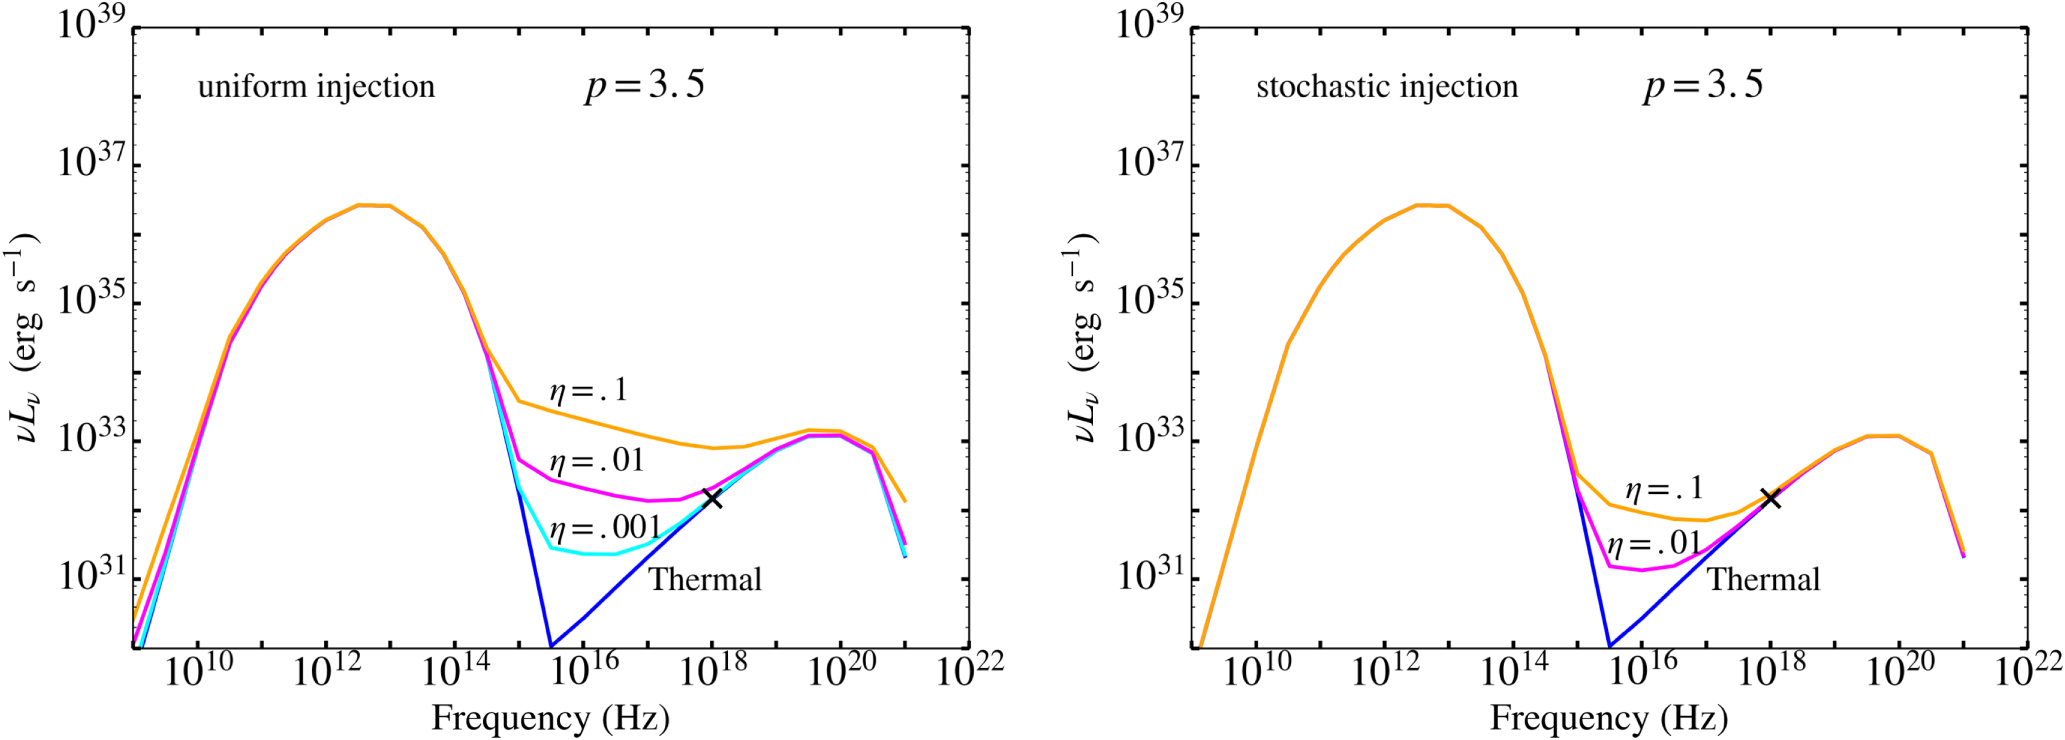
\includegraphics[angle=0,width=\columnwidth]{paper1_fig1}
\caption{Left: Spectra computed for quiescent (i.e., non-flaring) times for various values of the energy fraction of non-thermal electrons, $\eta$ with fixed power-law index, $p=3.5$, as well as for the purely thermal model.  In this configuration where the non-thermals only follow the thermal energy, the observed quiescent X-ray flux at $10^{18}$ Hz (depicted with an X) is exceeded even for moderate values of $\eta$.  Right: In this configuration, non-thermal electrons are injected in regions below $\beta=0.2$.  Localizing the non-thermal electrons to highly magnetized regions, where they are more likely to be accelerated, allows for significantly higher values of $eta$ while still accommodating the observed quiescent X-ray flux at $10^{18}$ Hz}
\label{fig1}
\end{figure}

In the right panel of Figure 1, we show the spectrum from the nonuniform stochastic model, where nonthermal electrons are localized to low-$\beta$ regions, again
with a power-law index of 3.5. Because of this localization, it is possible to accommodate higher fractions
of non-thermal electrons while still matching the quiescent thermal spectrum. In this model, it is possible
to inject almost 10\% of the total thermal energy into a
non-thermal electron distribution within the magnetized regions.
\section{X-Ray Variability: Stochastic Injection}


\begin{figure}
	\centering
	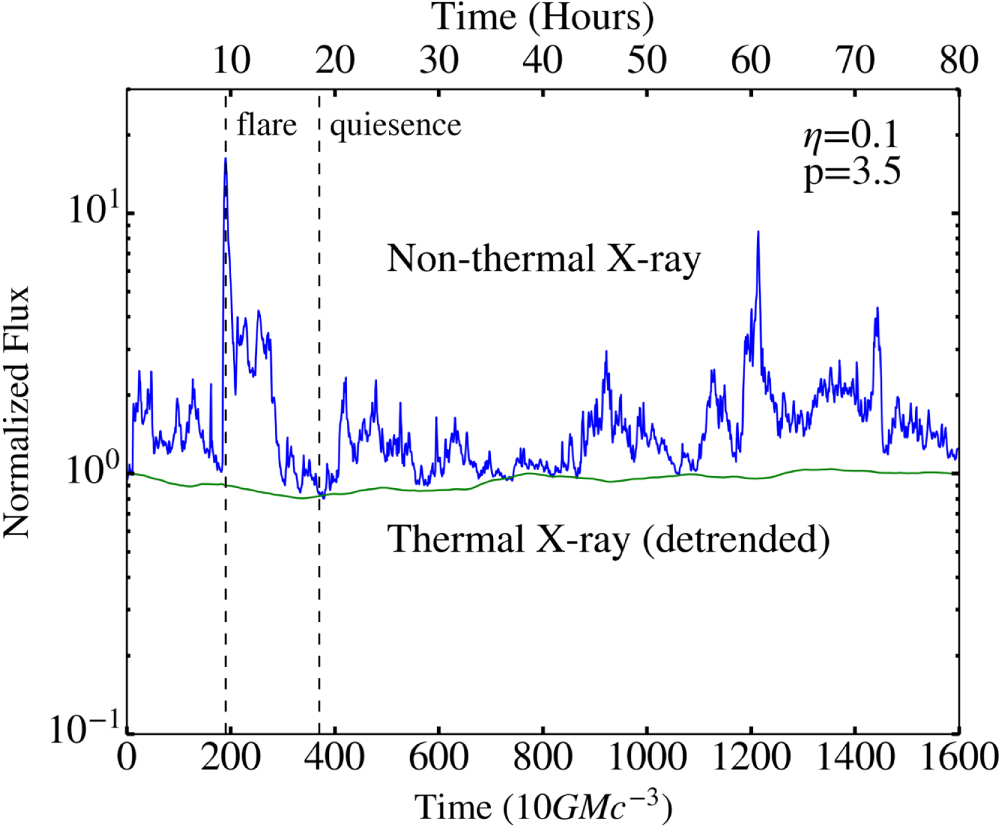
\includegraphics[angle=0,width=\columnwidth]{paper1_fig2}
	\caption{Thermal and non-thermal X-ray lightcurves.  The injection of non-thermal electrons into highly magnetized regions naturally produces significant variability due to the dynamic nature of magnetic fields in the accretion flow.}
	\label{fig2}
\end{figure}


\begin{figure}
	\centering
	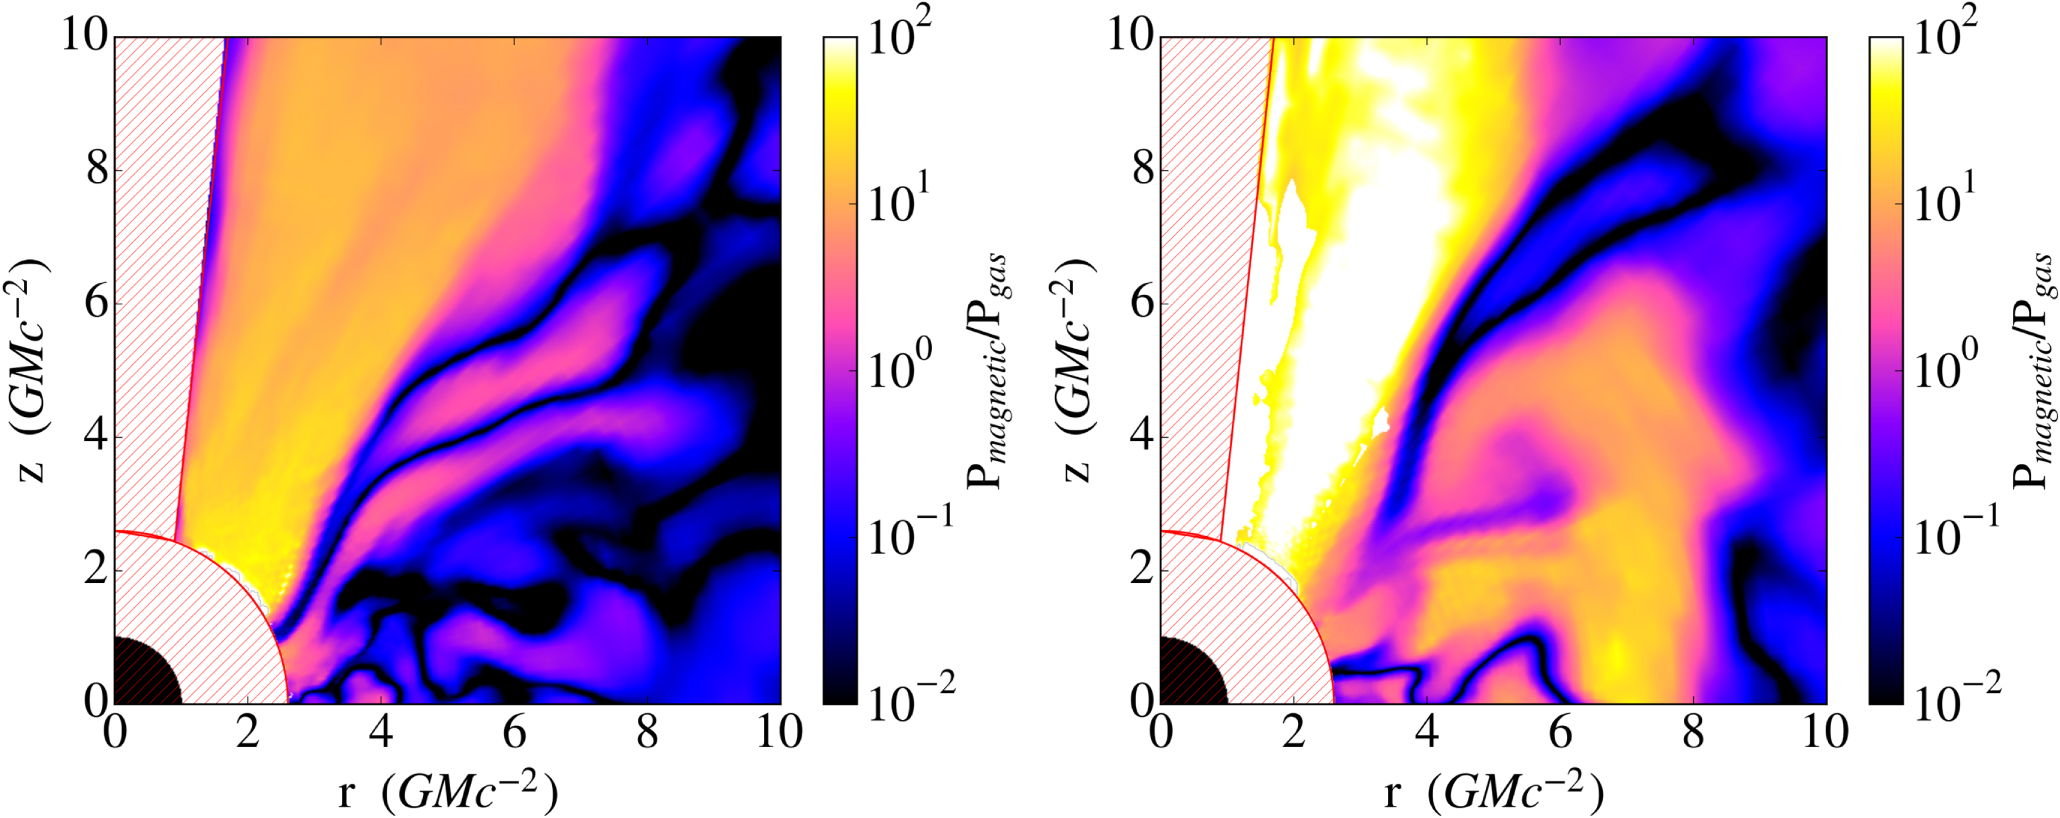
\includegraphics[angle=0,width=\columnwidth]{paper1_fig4}
	\caption{Left: Map of the ratio of the magnetic to gas pressure during a quiescent state in the simulation.  Cells near the pole and within the ISCO at $\sim 2.4 GMc^{-2}$ are excised due to numerical artifacts often occurring within these regions.  The black quarter-circle at the origin is the event horizon of the black hole.  Right: A large flux tube is present in the accretion flow during this flare, with high magnetization, resulting in a high ratio of pressures throughout a large portion of the disk. }
	\label{fig3}
\end{figure}

\begin{figure}
	\centering
	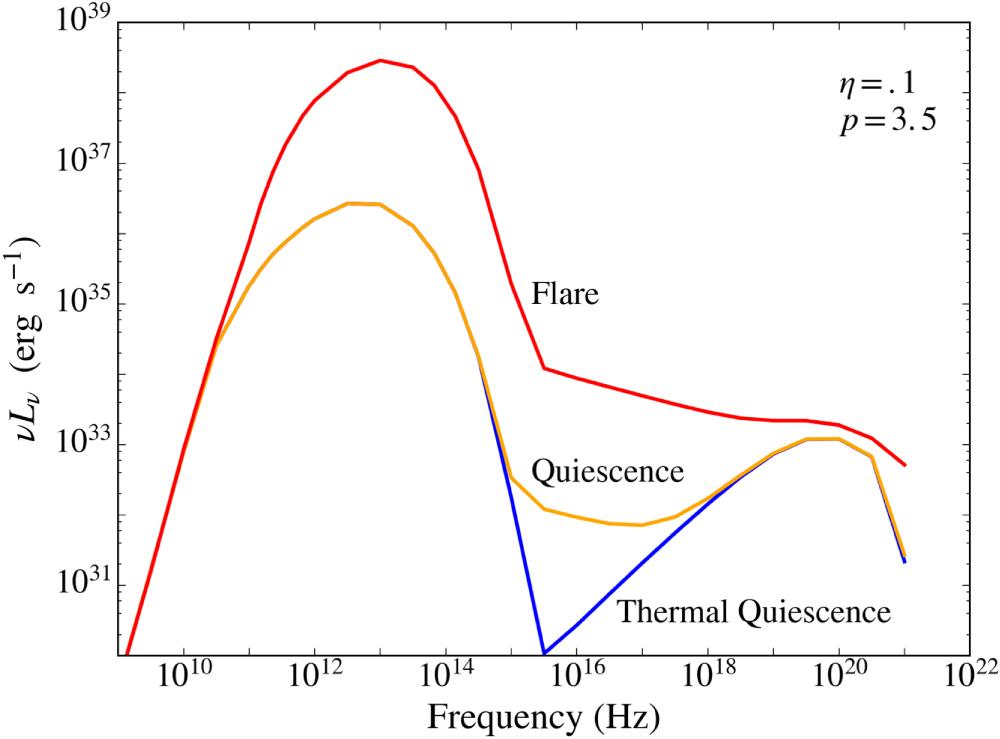
\includegraphics[angle=0,width=\columnwidth]{paper1_fig3}
	\caption{Spectra of the flaring and quiescent states depicted in Figure 3 in red and orange, respectively.  The purely thermal quiescent spectrum is shown for reference in blue. }
	\label{fig4}
\end{figure}

\begin{figure}
	\centering
	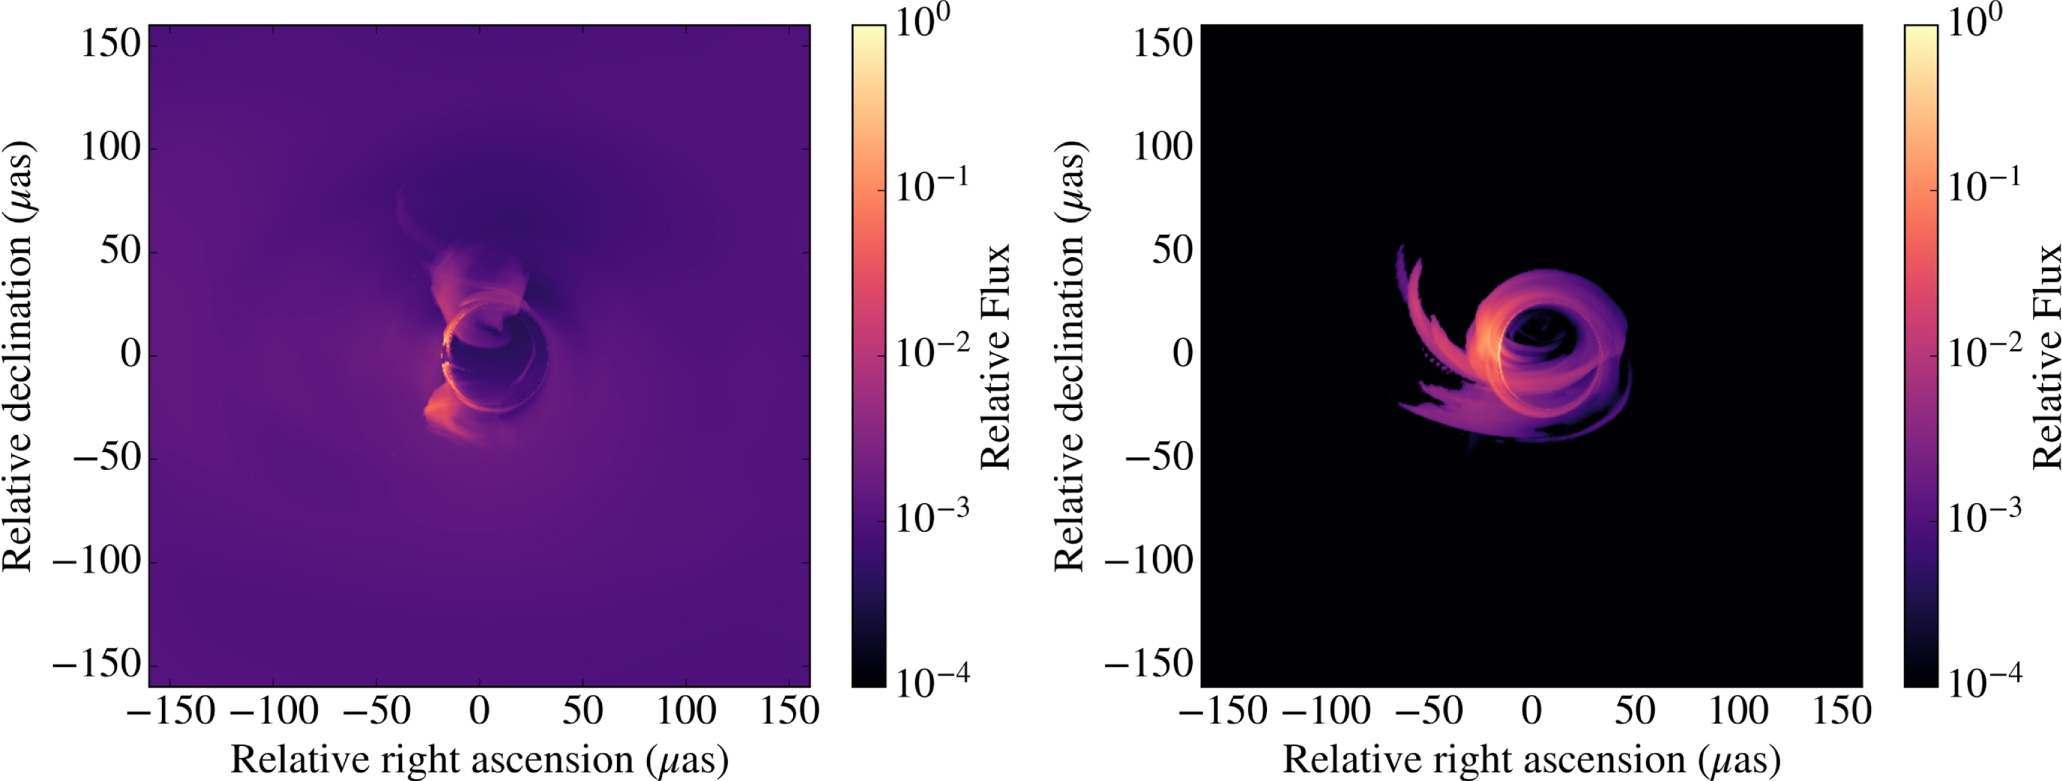
\includegraphics[angle=0,width=\columnwidth]{paper1_fig5}
	\caption{Left: Simulated image of quiescent X-ray (4.1 keV) emission. Fluxes are normalized to the maximum pixel value. Some
		structure is visible in the innermost regions of the image, where strong magnetic fields in the funnel close to the event horizon have
		associated non-thermal particles, and hence strong X-ray emission. We see that the extended Brehmsstrahlung emission comprises a
		significant fraction of the total flux during quiescence. Right: During the flare, emission is heavily dominated by the innermost part of the
		accretion flow; the relative contribution from the halo of Bremsstrahlung emission is negligible during flares.}
	\label{fig5}
\end{figure}

Apart from providing a more natural match to quiescent-state constraints, another interesting result
of using the $\beta$-dependent description of non-thermal electron injection is that it produces significant X-ray
variability. Perhaps this is not surprising, since the non-thermal electrons will trace magnetic flux tubes,
which are dynamic structures, constantly being formed, sheared, and moving throughout the flow. If one of these
flux tubes crosses a caustic behind the black hole, it will result in an additional amplification of the flux, and
since these tubes are emitting primarily non-thermal synchrotron radiation in the X-rays, they will cause X-ray
flares. We explore this variability in Figure \ref{fig2}, where we show the effect of stochastic injection of non-thermal electrons and compare it to a purely thermal model. In the nonthermal lightcurve, we see both persistent variability as
well as 4 large flares during the $\sim$80 hours of simulation. In the largest flares, the flux increases by a factor of $\sim 10$
compared to quiescence. The magnetically dominated regions responsible for these flares live for about 5000
seconds, which sets the timescale of the flares in this figure. There is indeed a stark contrast between this
result, which takes into account acceleration in low-$\beta$ regions, and the purely thermal model, which shows no variability.  We now investigate the properties of the magnetic structures in the innermost regions of the accretion flow
to further pinpoint the localization and time evolution of the flares. Figure \ref{fig3} shows the ratio of the magnetic
to the gas pressure throughout the inner flow during a
quiescent state and during the strongest flare from the
simulation. We see that this flare is caused by a large
magnetic flux region developing in the flow with $\beta < \beta_t$.
Due to the large spatial extent of this tube, many nonthermal electrons are injected, causing a sudden increase
in the X-ray flux. In contrast, during quiescence, the only
region with a significant number of non-thermal electrons
is in the funnel, which typically has a fairly uniform and
strong magnetic field. This only contributes a small flux
and results in low level variability.
Figure \ref{fig4} depicts the spectra of the flaring and quiescent
states from the simulation. During quiescence, the nonthermal emission is not especially prominent; its nature is
largely obscured by the thermal emission dominating at
most wavelengths. During the flare, however, the powerlaw nature of the non-thermal emission becomes more
evident.
In Figure 5, we show the X-ray images of our model
during flaring and quiescent states. The images show
the relative contribution to the overall flux from various
parts of the accretion flow. During quiescence, we find
that while there is some contribution to the X-ray flux

from a small population of non-thermal particles in the
funnel, the extended Bremsstrahlung emission accounts
for the majority of the total (i.e., integrated over the entire image) observed flux. During a flare, the emission is
heavily dominated by non-thermal electrons in the inner
accretion flow, rendering the Bremsstrahlung flux negligible. The difference in the localization of the X-rays
between the non-thermal and thermal models is responsible for their different variability properties.

\section{Comparison to Observations}
By interpreting observations of Sgr A* in the context of our GRMHD simulations, we begin to place constraints on the population of non-thermal electrons in the radiatively inefficient accretion flow and gain insight into their injection mechanisms. We employed two configurations for non-thermal electron injection, one in which the non-thermal electrons simply track the thermal energy everywhere throughout the flow and another where the non-thermal electrons are injected solely into regions of high magnetization. From the first model we are able to place tight constraints on the fraction of steady-state non-thermal electrons that may exist throughout the flow by comparing the simulations to the observed quiescent X-ray flux. The second model localizes non-thermal electrons to a much smaller region, allowing their local energy density to be much higher than the uniform model (by about 2 orders of magnitude) while still matching the
observed quiescent X-ray flux.


We find that X-ray variability is a generic result of constraining the non-thermal electrons to highly magnetized regions. This is because the magnetic field is
dynamic throughout the flow, generating magnetic flux tubes, which are in a constant state of being formed, sheared, becoming buoyant, and leaving the disk. The
dynamic nature of these flux tubes combined with strong lensing effects from the black hole generate both persistent variability as well as flaring events.
X-ray flares in our simulations are always coincident with IR flares, but there are numerous IR flares without
X-ray counterparts, as shown in Figure 8, which qualitatively matches observations. In this figure, we have zoomed in to the first 250 timesteps of the simulation in order to more clearly illustrate the relationship between the IR and X-ray lightcurves. During this time span,
we observe about 5 IR flares over the stochastically variable background and one significant X-ray flare. From our simulation we find that there are about 5 IR flares per X-ray flare and a rate of one X-ray flare per 72,000 seconds, over the entire simulation. Over the course of
3 million seconds of observation with Chandra, 39 Xray flares were observed, corresponding to one flare every $\sim$77,000 seconds. Observations Sgr A* show that,
for every X-ray flare, there are about 4 NIR flares (e.g., Genzel et al. 2003; Eckart et al. 2006). These numbers
are in rough agreement with our results. In order to compare flare statistics from our simulations to observations more directly (e.g., through flux
distributions reported in Neilsen et al. 2015), we need to account for the fact that only  $\sim 10\%$ of the X-ray
emission from Sgr A* comes from the inner accretion flow (Neilsen et al. 2013). In Figure 9, after adding a
constant background equal to 90\% of the observed quiescent flux to our lightcurve from Figure 2, we plot the
flux distribution in our simulations. We find that the flare distribution resembles a power-law with an index of
around 2.3, while the lower-level variability does not have an obvious structure. Neilsen et al. (2015) reports only
Poisson variability at low fluxes, and power-law behavior at high fluxes, with a power-law index of 1.92. This is
roughly consistent with our simulated flux distribution. Our simulations, however, do not account for the Poisson photon counting noise, and also do not show as large of a range of variability. The latter is likely due to the
relatively short duration of our simulation that did not capture many rare, high flux events.
We estimate the level of the Poisson noise, below which we expect our simulated flux distribution to deviate significantly fom observations. We take the reported photon counting rate ($Q = 5.24$ cts/ks) and binning ($b = 300$ s) from Neilsen et al. (2015) and calculate the typical fractional Poisson error, $\epsilon=1/\sqrt{Qb}=0.79$. Normalizing our lowest level of emission to 1, we see that counting noise
will dominate the observed variability from 1 to $1+\epsilon$,
setting the lower limit from which we expect our simulations to reproduce the flux distribution.
We further explore the relationship between IR and Xray fluxes in Figure 10. The largest IR flares correspond
to the largest X-ray flares, but there is much more variability in the IR than the X-rays. In our simulations,
anytime a flux tube appears and crosses a caustic there
will be an IR flare due to the synchrotron emission from
the thermal electrons. However, only the most highly
magnetized flux tubes will have non-thermal electrons
associated with them and will generate an X-ray flare.
The effect of the $\beta$ threshold is to pick out a subset of all
the magnetic flux tubes, ones with conditions suitable for
reconnection to occur. The particular threshold we use is
motivated by Li et al. (2015a), who showed a non-thermal
component being generated for $\beta < 0.2$. As a result, IR
variability is much more significant, since there is thermal synchrotron associated with all flux tubes, whereas
particle acceleration and hence X-ray emission only occurs for a particular subset of the tubes. Additionally,
we see that the flux tubes responsible for the largest IR
flares are the same structures responsible for the largest
X-ray flares. This is unsurprising given the strong scaling
of synchrotron emissivity with magnetic field; the most
highly magnetized flux tubes radiate copiously in the IR
due to the high magnetic fields, and also act as sites of
efficient reconnection, generating strong X-ray flares.
\section{Conclusions}